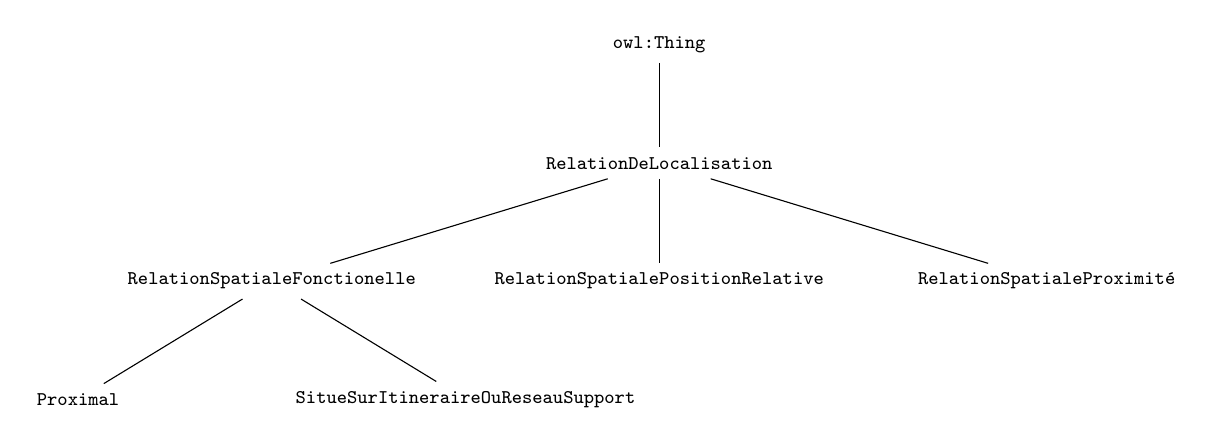
\begin{tikzpicture}[
  man/.style={rectangle,draw,fill=blue!20},
  woman/.style={rectangle,draw,fill=red!20,rounded corners=.8ex},
  grandchild/.style={grow=down,xshift=1em,anchor=west,
    edge from parent path={(\tikzparentnode.south) |- (\tikzchildnode.west)}},
  first/.style={level distance=6ex},
  second/.style={level distance=12ex},
  third/.style={level distance=18ex},
  level/.style={font=\scriptsize\ttfamily},
  level 1/.style={sibling distance=14em}]
  % Parents
  \node[level]{owl:Thing}
  child{node {RelationDeLocalisation}
    child{node {RelationSpatialeFonctionelle}
      child{node{Proximal}}
      child{node{SitueSurItineraireOuReseauSupport}}
    }
    child{node {RelationSpatialePositionRelative}}
    child{node {RelationSpatialeProximité}}
  };
\end{tikzpicture}